\chapter{Radar system documentation} \label{app:docs}

In this appendix, it is attached the most up-to-date documentation for the developed radar system.

\begin{table}[h!]
	\centering
	\begin{tblr}{
			width = \linewidth,
			colspec = {Q[88]Q[125]Q[725]},
			hline{1,6} = {-}{0.08em},
			hline{2} = {-}{},
		}
		\textbf{Version} & \textbf{Date} & \textbf{Comment}\\
		1 & 29/06/2022 & Initial release\\
		2 & 21/08/2022 & Added additional documentation for micro-Doppler operation mode\\
		3 & 16/11/2022 & Added programming requirements documentation\\
		4 & 27/12/2022 & Added DSP code description and installation steps. Corrected folder names
	\end{tblr}
\end{table}

\paragraph{Summary}
\textit{This document serves as documentation for the different working parts of the Zenith BLE Radar Processing System, a hardware, firmware and PC application to enable the operation of a real-time CWLFM radar processing system with a focus on gait analysis.}

\section{Introduction} \label{secdoc:Introduction}

Zenith BLE is a radar processing firmware and PC application that enables the wireless acquisition and processing of CWLFM radar samples for the purpose of gait analysis. The solution consists of two parts: a modifiable firmware for use with BLE-enabled STM32 MCUs and two stand-alone PC executables to use with a PC with a pre-installed or external Bluetooth card.

This documents outlines the different parts of the system, the procedure to install the firmware and run the PC applications, the means to apply common and simple modifications to the firmware and the PC applications and some guidance on further modifications.

\section{System requirements}

The system requirements for the different parts comprise the physical node and the PC that runs the application. To configure and program the node several components must be present in a programming PC. In this section these tools are outlined and described.

\subsection{Physical node}

The physical node is a PCB layout that embeds the STM32WB15CC MCU which features a 10-pin JTAG connector as shown in \cref{fig:jtag}.  To program the physical node, two software components must be present on a Windows PC.

\begin{figure}[ht]
	\centering
	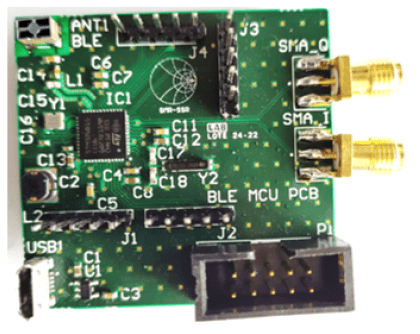
\includegraphics[width=0.6\linewidth]{jtag.png}
	\caption{Main MCU PCB with JTAG connector \label{fig:jtag}}
\end{figure}

\subsubsection{STM32CubeIDE}

To modify the source code of the firmware and program the MCU, STM32CubeIDE must be present in the PC. To download the STM32CubeIDE software, head over to \url{https://www.st.com/en/development-tools/stm32cubeide.html}. An image of the main interface of STM32CubeIDE is found in \cref{fig:ide_main}.

\begin{figure}[ht]
	\centering
	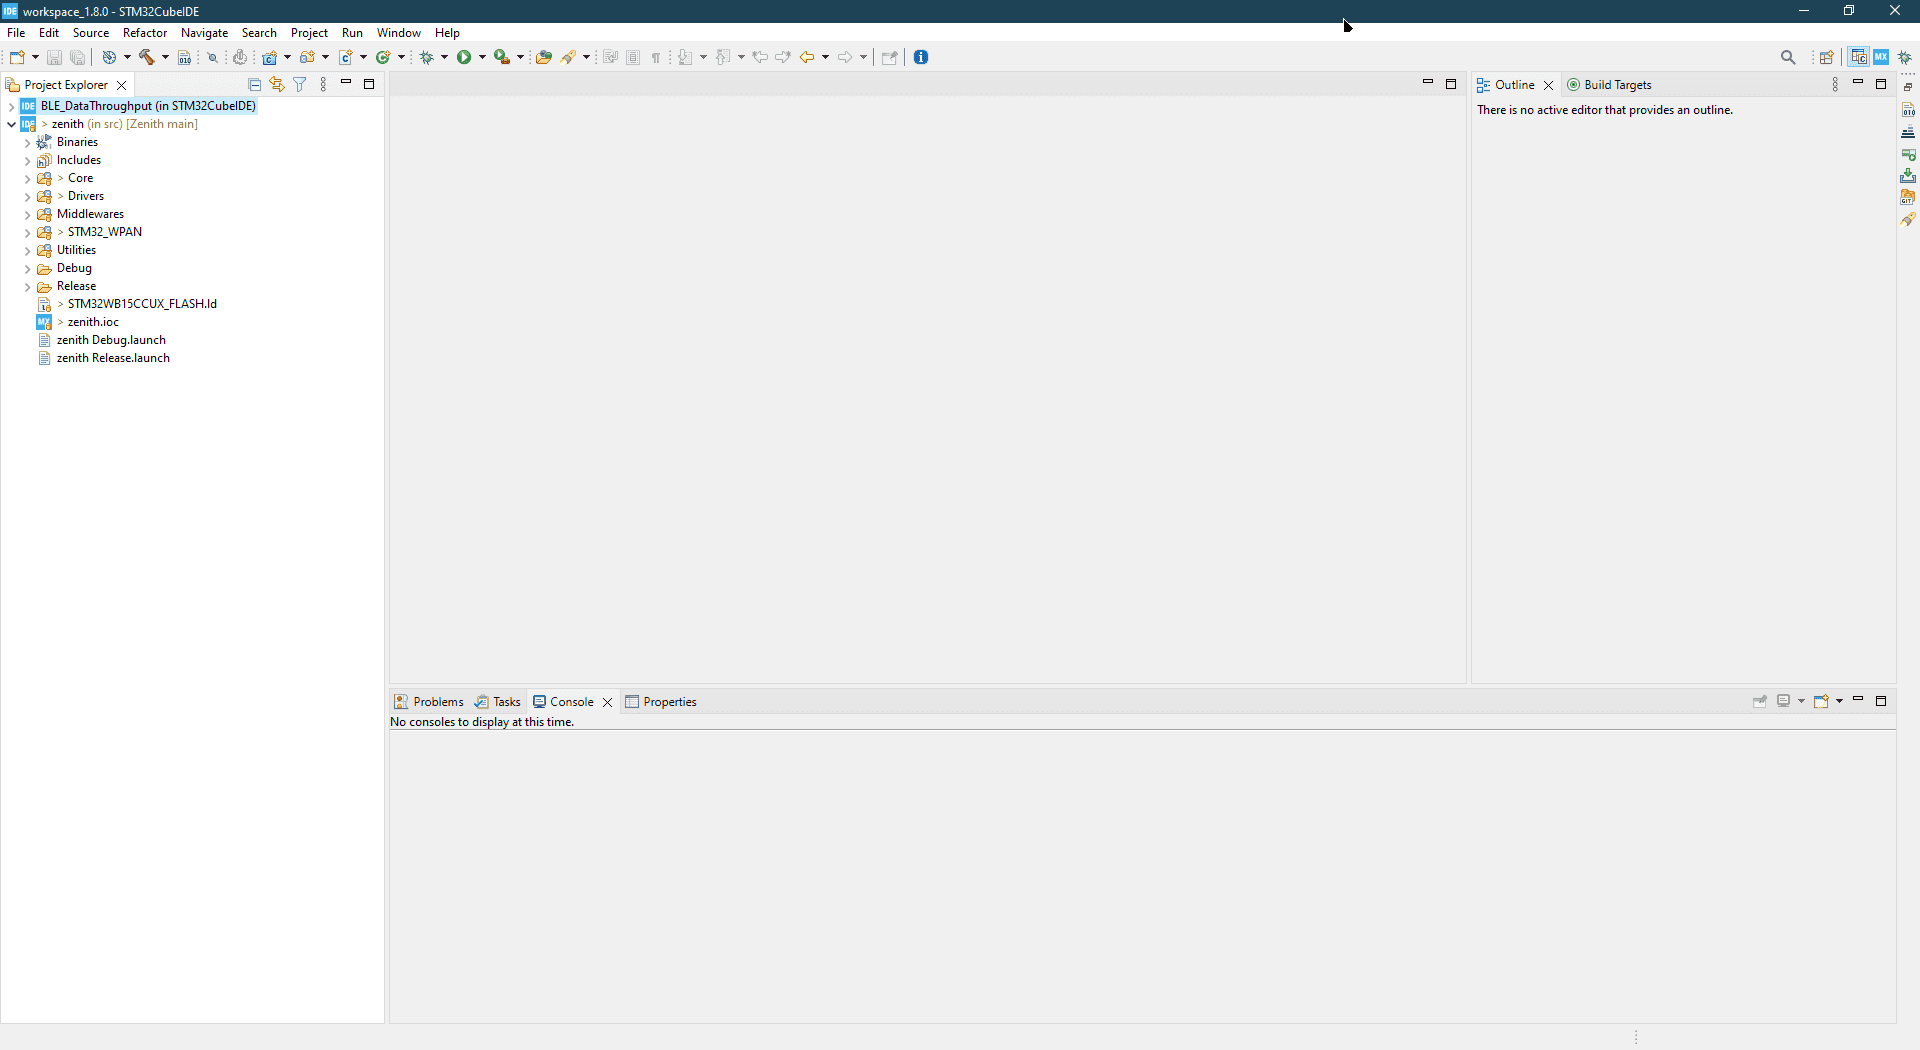
\includegraphics[width=\linewidth]{ide_main_if.png}
	\caption{STM32CubeIDE main interface \label{fig:ide_main}}
\end{figure}

\subsubsection{STM32CubeProgrammer}

To debug the low-level operation and register control of the MCU, it is advisable that it is also downloaded and installed the STM32CubeProgrammer software at \url{https://www.st.com/en/development-tools/stm32cubeprog.html}. An image of the main interface of STMCubeProgrammer is found in \cref{fig:prog_main}.

\begin{figure}[ht]
	\centering
	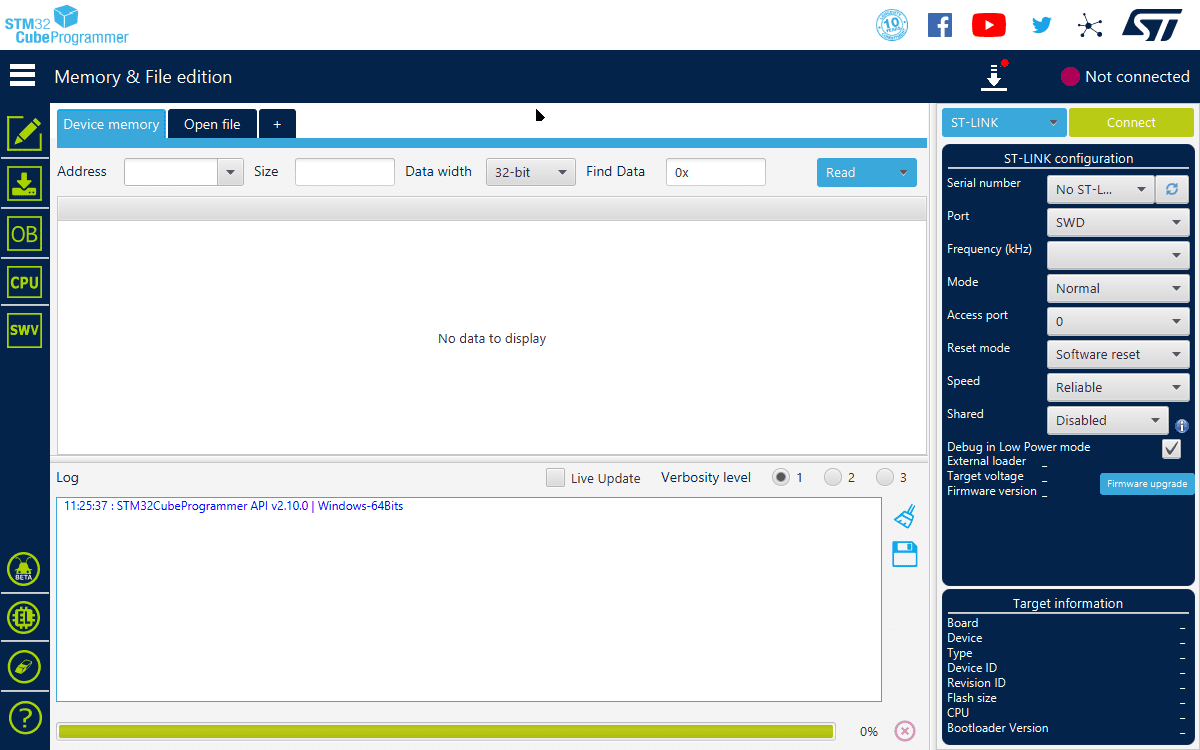
\includegraphics[width=\linewidth]{programmer_main_if.png}
	\caption{STM32CubeProgrammer main interface \label{fig:prog_main}}
\end{figure}

\subsubsection{ST-Link}

In order to program the MCU, it is necessary to attach the JTAG connector of the ST-Link to the JTAG debug receptacle in the MCU PCB.

\subsection{PC applications} \label{secdoc:pc_install}

The PC applications need some software and dependencies to run, as well as installing and running the dependencies. In this section, the installation procedure of the PC applications is outlined.

\subsubsection{Python}

The PC applications are programmed with the \textit{Python} programming language. The PC applications have also some dependencies. The dependencies are installed and managed using a dependency management system described in \cref{secdoc:pipenv}. The minimum Python version needed to run the PC applications is Python 3.9.1. To download and install Python in a PC follow the instructions in \url{https://www.python.org/downloads/}.

\subsubsection{Pipenv} \label{secdoc:pipenv}

\textit{Pipenv} is the dependency management system to handle the installation of the required dependencies for the PC applications. To download and install Pipenv, first install Python and then run:

\begin{minted}{bash}
pip install --user pipenv
\end{minted}

After the installation finishes, navigate with the CMD (Windows Command Prompt) to inside the PC application folder (the PC application folder is called \textit{pc\_app\_ble\_epsilon\_vYYYYMMDD}). Make sure that a \textit{Pipfile} file is present in the folder, then execute the following command:

\begin{minted}{bash}
pipenv install
\end{minted}

The documentation of Pipenv is located at \url{https://pipenv.pypa.io/en/latest/}.


\section{Firmware preparation}

Once STM32CubeIDE is present on the system, the project can be imported from the \texttt{.zip} file containing the project source code. From a fresh installation of STM32CubeIDE select the location of your workspace at the \textit{Launcher} window (\cref{fig:ide_wk}) and click on \textit{Launch}. After the instantiation of the workspace, a window with the editor will appear (\cref{fig:ide_first}).

\begin{figure}[ht]
	\centering
	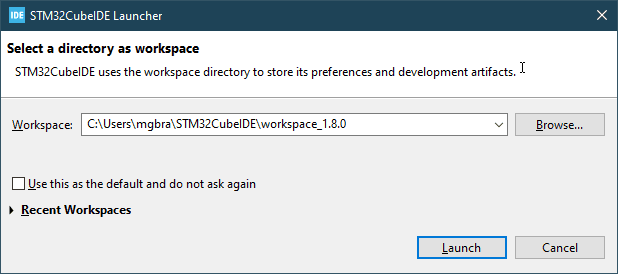
\includegraphics[width=0.8\linewidth]{ide_wk.png}
	\caption{STM32CubeIDE workspace launcher \label{fig:ide_wk}}
\end{figure}

\begin{figure}[ht]
	\centering
	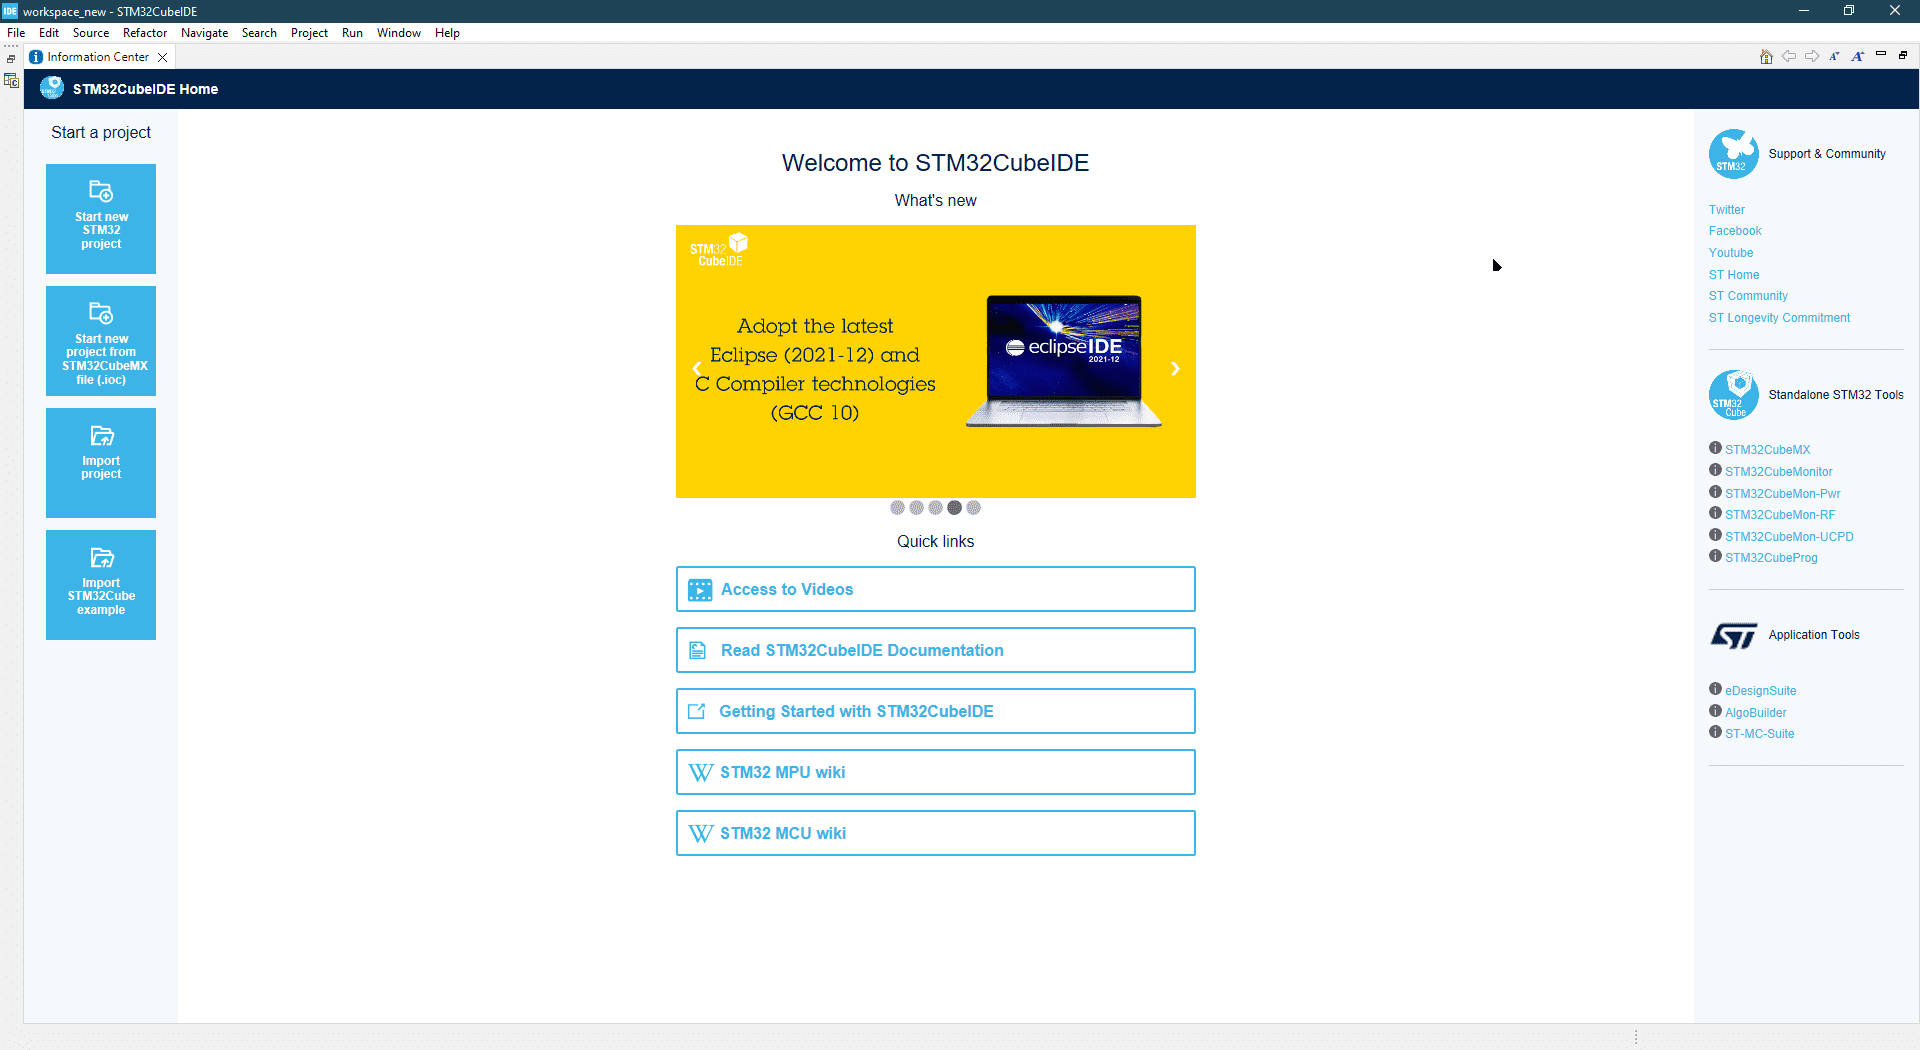
\includegraphics[width=\linewidth]{ide_first.png}
	\caption{STM32CubeIDE first launch \label{fig:ide_first}}
\end{figure}

\subsection{Importing the project}

To import the firmware project that is in \texttt{.zip} format, click \textit{File » Open Projects from File System...} and click the \textit{Archive...} button. Navigate and select the archive file containing the last version of the firmware. The window will populate with the project information and files as shown in \cref{fig:ide_import}. Select only the entry with the import type of \textit{Eclipse project}. Then click \textit{Finish}.

\begin{figure}[ht]
	\centering
	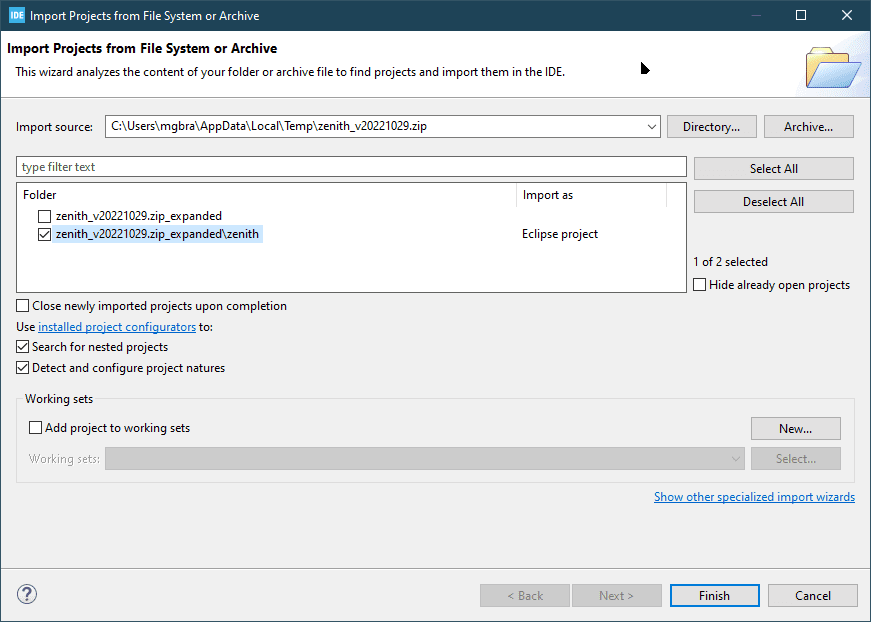
\includegraphics[width=0.8\linewidth]{ide_import.png}
	\caption{STM32CubeIDE import project from archive dialog \label{fig:ide_import}}
\end{figure}

Close the \textit{Information Center} the project will appear in the left panel. The IDE application is now ready to make modifications and build the firmware.

\subsection{Folder structure}

The project is structured in the following way:
\begin{itemize}
	\item \textit{Binaries}: contains the built binaries from the compilation of the project. If the compiled binary firmware is wished to be shared, the executable binary can be found here.
	\item \textit{Includes}: contains the bundled header files from the compilation of the project
	\item \textit{Core}: where the main source code resides
	\begin{itemize}
		\item \textit{Inc}: header files that are modifiable corresponding to different source files
		\item \textit{Src}: the main \textit{.c} source files of the project.
		\item \textit{Startup}: MCU startup assembly execution files (rarely need to be modified).
	\end{itemize}
	\item \textit{Drivers}: contains the DSP and FPU drivers of the system with some modifications for operation with the radar signals (rarely need to be modified).
	\item \textit{Middlewares}: additional software support for communication middleware stacks. Contains BLE drivers.
	\item  \textit{STM32\_WPAN}: source files and routines of the BLE communicationpart of the project.
	\begin{itemize}
		\item \textit{App}: source and header files of the BLE code running in the BLE co-processor.
		\item \textit{Target}: interface with the inter-process communication controller for the MCU (not modifiable).
	\end{itemize}
	\item \textit{zenith.ioc}: MCU peripherals and clock configuration file.
\end{itemize}

The main of potential modifications are done under \textit{Core} (\textit{Inc} and \textit{Src}) and \textit{App} folder under \textit{STM32\_WPAN}.

Under \textit{Inc} and \textit{Src}, there are source and header files for every peripheral so that their configuration can be seen independent to other peripheral and easier to navigate.

\subsection{MCU core and peripheral configuration}

The firmware is designed so that is rarely necessary to make modifications directly to the peripherals or the core systems of the MCU. However, if needed one can make such changes in the \textit{zenith.ioc} file. As these changes are not necessary for the operation of the radar processing system, they are not covered in this documentation. An illustration of the interface of the \textit{zenith.ioc} file is shown in \cref{fig:ide_ioc}.

\begin{figure}[ht]
	\centering
	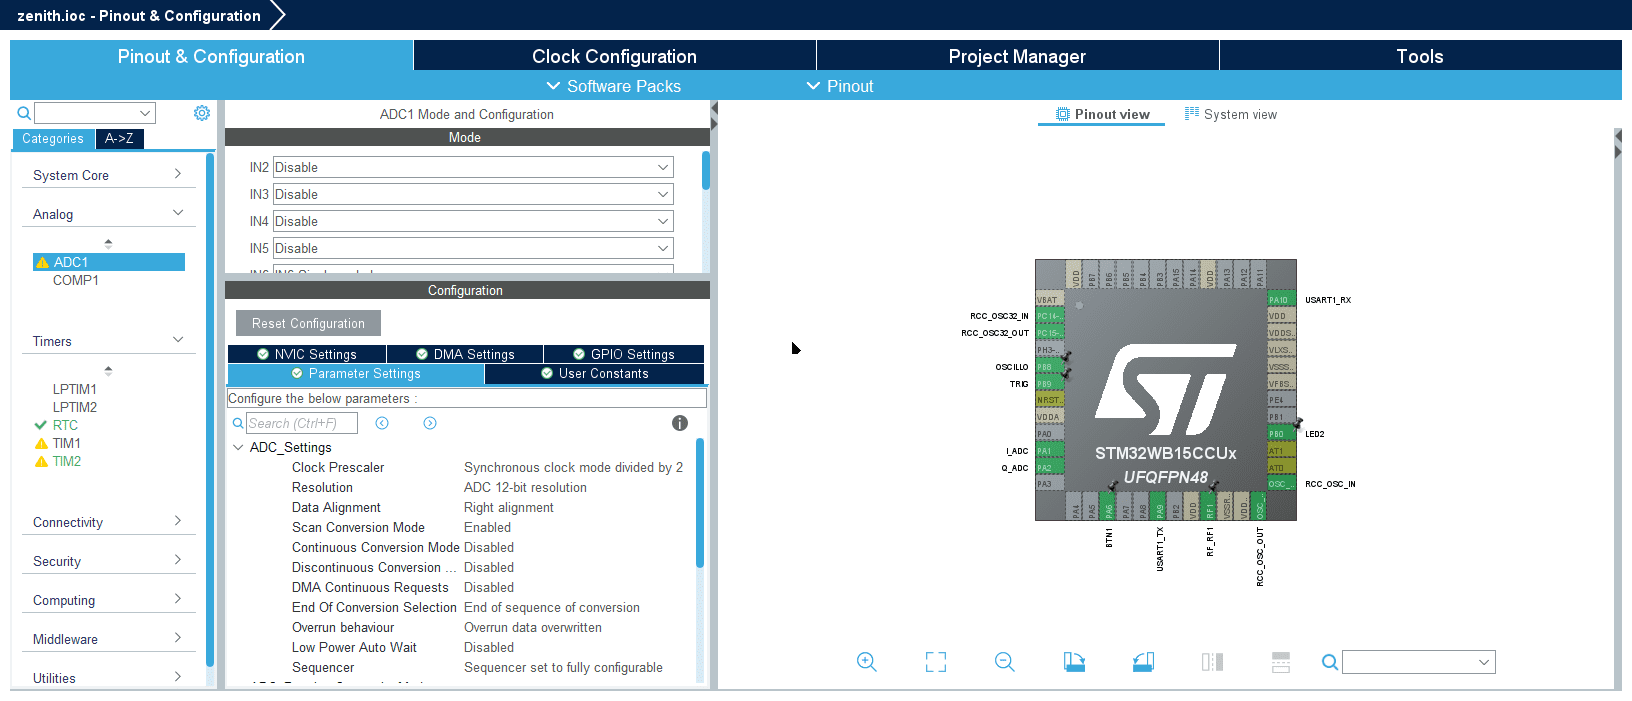
\includegraphics[width=\linewidth]{ide_ioc.png}
	\caption{IOC file edition under STM32CubeIDE \label{fig:ide_ioc}}
\end{figure}

\section{Main modifications to the firmware}

To change the operation of the firmware, for instance to match a different chirp time of the CWLFM signals, some modifications need to be performed.

\subsection{Modification of the ADC sample rate}

The sample rate of the ADC must be changed to allow a correct sampling of the CWLFM signals depending on the chirp time. Changing the working frequency of the ADC is simple: in \textit{Core » Inc » tim.h} the following two lines control the clock of the ADC:

\begin{minted}{c}
#define TIMER2_FREQUENCY_HZ              (fU)
#define TIMER2_FREQUENCY_RANGE_MAX_HZ    (fU)
\end{minted}

In the previous listing, \texttt{f} stands for the desired working frequency of the ADC in Hz.
\texttt{U} stands for \textit{unsigned integer}. This suffix is added to constant values in the source to explicitly state that they are positive integers. This acts an additional security measure to only allow the program to compile if \texttt{f} is a positive integer. Due to constraints of the ADC peripheral, $f \le 34000000$.

Taking into account that the sampling of the two channels of the ADC is done sequentially, the numbers defined should be twice the desired sampling frequency for each channel (I or Q respectively). For instance, to achieve a sampling rate of 125 ksps for I and Q, \texttt{f} should be set to 250000.

%exmple%

\subsection{Modification of the sampling and processing operations}

The sampling and processing operations have common configurations and configurations only effective under micro-Doppler enabled capabilities or normal operation. The common configurations are first outlined in this subsection. All configurations are performed in the \textit{Core » Inc » main.h} file.

\subsubsection{Adjusting sampling buffer size}

The buffer that is used to store the samples of the signal must be sufficiently big to hold the values for the sampling of one ramp. Therefore its size needs to be adjusted.

The size of the array can be calculated with the following formula:
\begin{equation} \label{eqn:s_value}
	s = \lceil 2 f_s T_c \rceil
\end{equation}
Consequently, the value must be adjusted in the following line, where \texttt{s} is the computed value according to \cref{eqn:s_value}:
\begin{minted}{c}
#define ADC_CONVERTED_DATA_BUFFER_SIZE   (1UL*sU)
\end{minted}

In the previous listing, \texttt{UL} stands for the data type \textit{unsigned long} and \texttt{U} for \textit{unsigned integer}. These suffixes are added to constant values in the source to explicitly state that they are positive integers of a maximum of 32 bits. This size limitation is due to the word size of the STM32 architecture. This acts an additional security measure to only allow the program to compile if \texttt{s} is a positive integer within the range $[0, 2^{32} - 1]$ and the array fits into the maximum free memory available. The available memory depends on the size of the FFT configured, by default is 256. Under these conditions $s \le 1312$.

For example, for a $T_c = \SI{625}{\micro\second}$ and $f_s = \SI{125}{\kilo sps}$, the obtained size value is $s = 157$, as can be seen configured in the line above.

A new version is being developed where these parameters are computed automatically at compile time, being the only configurable parameters $T_c$ and $f_s$.

%example with code%

\subsubsection{Adjusting BLE packet queue size}

The samples are sent in BLE packets of 247 bytes. A queue system to store packets to be sent has been developed and the size of the queue can be adjusted. It is currently set to the maximum possible in order to optimize throughput and maximise available memory. Nonetheless, it can be changed by modifying the following line:
\begin{minted}{c}
#define QUEUE_BLE_PACKETS_NO 22 /* max 22 packets in the queue */
\end{minted}

In every packet, the DSP data from one or several ramps (see next section) is sent along with an ID number. This ID number is used to identify packets and therefore ramps. The ID number is contained in the last 2 bytes of the data payload in each packet.

\subsubsection{Configuring bin sending properties}

The resulting FFT bins that are sent can be adjusted according to specific needs. The lines that control these characteristics are:
\begin{minted}{c}
#define SEND_BIN_NO 20
#define BIN_SENT_OFFSET 3
#define SEND_BIN_INITIAL_IDX 0
\end{minted}
The different variables control different aspects:
\begin{itemize}
	\item \texttt{BIN\_SENT\_OFFSET} controls the ramps that are sent per packet. This can be adjusted but is currently configured to optimize throughput and maximise available memory.
	\item The bins sent can be controlled via \texttt{SEND\_BIN\_INITIAL\_IDX} and \texttt{SEND\_BIN\_NO} such that the bins that will be sent to the PC application are [\texttt{SEND\_BIN\_INITIAL\_IDX}, \texttt{SEND\_BIN\_INITIAL\_IDX} + \texttt{SEND\_BIN\_NO} - 1] inclusive. This will need to match the PC application configuration.
\end{itemize}

These values must follow a restriction imposed by the maximum number of bins a packet can hold, which is 61. The can both be freely configured as long as the following condition is held:
\begin{equation}
	\mathtt{BIN\_SENT\_OFFSET} \cdot \mathtt{SEND\_BIN\_NO} \le 61
\end{equation}

\subsubsection{Configuring the rejection of extrema ramp samples}

The quantity of samples that are rejected from the ends of a sampled ramp can be configured as well. The lines that control this configuration are:
\begin{minted}{c}
#define EXTREMA_SAMPLES_DISCARD_NO 16
#define TOTAL_SAMPLES_DISCARD_NO 48
\end{minted}
The number of samples that will be discarded are as follows:
\begin{itemize}
	\item From the left (initial) side of the sampled ramp: $\texttt{EXTREMA\_SAMPLES\_DISCARD\_NO}$.
	\item From the right (final) side of the sampled ramp: $\texttt{TOTAL\_SAMPLES\_DISCARD\_NO} - \texttt{EXTREMA\_SAMPLES\_DISCARD\_NO}$.
\end{itemize}

\subsubsection{micro-Doppler operation mode} \label{secdoc:micro_doppler_operation}

The micro-Doppler operation mode involves a summation of bins and slightly changes the processing pipeline. The micro-Doppler operation mode is activated if the following line is present in the header file:
\begin{minted}{c}
#define MICRODOPPLER_MODE
\end{minted}

In this scenario, several further configurations are available:
\begin{minted}{c}
#define MD_BIN_SUM_START 10
#define MD_BIN_SUM_NUMBER 60
#define MD_SUMS_PER_PACKET 30 /* max 30 ramps */
\end{minted}

This controls the bins that are summed and the bins that are sent per packet. The bins that are summed can be controlled with variables \texttt{MD\_BIN\_SUM\_START} and \texttt{MD\_BIN\_SUM\_NUMBER} such that the bins that will are summed are \texttt{MD\_BIN\_SUM\_NUMBER} bins starting from bin \texttt{MD\_BIN\_SUM\_START}, inclusive.

\texttt{MD\_RAMPS\_PER\_PACKET} controls the number of sums that are sent in each packet, each BLE packet is not sent until all sums that fit in that packet are computed. This controls the available sums to work with in the PC application. It is configured as the maximum permissible to maximise throughput.

\section{Firmware DSP source code description}

The source code related to the DSP pipeline is explained here, so as to allow an understanding of the DSP processing stages and how a user can add or remove additional preprocessing stages.

The DSP routines are executed when an interrupt from the ADC is received indicating the end of a ramp sample. This interrupt calls the function \texttt{HAL\_ADC\_ConvCpltCallback} located in the \textit{main.c} file. Inside this function there are present the different stages of DSP routines that the data undergoes.

The data is stored and modified in the same data structure in static random access memory (SRAM), a vector of 16-bit unsigned integers called \texttt{uhADCxConvertedData}.

The implemented DSP routines are as follows:
\begin{enumerate}
	\item Extrema sample discard
	\item Q15 format conversion
	\item FFT computation
	\item Optional additional bin summation if micro-Doppler mode is active
\end{enumerate}

The DSP routines are implemented as sequential operations or function calls that modify the data present in the vector stored in SRAM. The pseudocode for the DSP routines implementation within the interrupt-called function \texttt{HAL\_ADC\_ConvCpltCallback} is the following:

\begin{minted}{c}
void HAL_ADC_ConvCpltCallback(ADC_HandleTypeDef *hadc) {
	sampleDiscard();
	q15Conversion();
	fftCompute();
	#ifdef MICRODOPPLER_MODE
	binSummation();
	#endif
	HAL_DMA_Start_IT(...);
}
\end{minted}

The last call corresponds to an instruction for the DMA to transfer the contents of memory to the BLE secondary processor, to assemble and send the BLE packets. It must not be modified if the purposes of source code modification is to add or remove DSP routines in the sequence of data processing.

The DSP routines can be implemented as function calls or as direct operations inside the functions such as loops or conditional branches. In the implemented version of the firmware, the extrema sample discard, the q15 conversion and the bin summation are implemented directly to optimise system execution time by not adding assembly subroutines or branching instructions. The FFT computation is done as a function call as it implements optimised assembly code that produces a faster FFT computation time.

\subsection{Extrema sample rejection/discard and Q15 format conversion}

The extrema sample discard and Q15 format conversion is done in a single step by iterating through the ADC samples vector. The variable is then renamed to \texttt{uhADCxConvertedData\_q15} to give indication that the data that the vector now holds is in Q15 format. This numbering format conversion, algorithm and extrema rejection step is further explained in the Bachelor Thesis related to the system development. The code that discards the samples and converts to the Q15 format is the following:

\begin{minted}{c}
for (uint16_t i = 0;
i < ADC_CONVERTED_DATA_BUFFER_SIZE - TOTAL_SAMPLES_DISCARD_NO;
i++) {
	uhADCxConvertedData_q15[i] =
	((int32_t)
	(uhADCxConvertedData[i + EXTREMA_SAMPLES_DISCARD_NO])
	* 65535U + 2047U) / 4095U - 32768U;
}
\end{minted}

\subsection{FFT computation}

The FFT computation is performed via a function call and a parameter selection. The parameter selection allows to choose the FFT size in powers of two. The current implemented size is 256. The code that performs the FFT computation is the following:

\begin{minted}{c}
arm_cfft_q15(&arm_cfft_sR_q15_len256,
(q15_t*) uhADCxConvertedData_q15, 0, 1);
\end{minted}

In this case, the size can be adjusted by changing the parameter in the first argument of the function \texttt{\&arm\_cfft\_sR\_q15\_lenNNN} where \texttt{NNN} should be substituted with the desired FFT size. The second parameter is a pointer to the vector containing the data in IQ interleaved format. This format is automatically achieved due to the configuration of the ADC sampling order and should not be altered. The third parameter is a \texttt{0}, indicating that the transform is a forward transform. The last parameter is a \texttt{1} indicating that the FFT results should be ordered in interleaved complex form where for every bin, the real and imaginary components are sequentially ordered in the vector. The ordering obtained as a result of the FFT computation is described in detail in the Bachelor Thesis related to the system development. After this function call, the \texttt{uhADCxConvertedData\_q15} vector contains the frequency bin information in complex form and in bin order.

\subsection{Optional micro-Doppler bin summation}

This step is implemented between a \texttt{\#ifdef} directive indicating that it should only compile if the micro-Doppler mode is active, accordingly, the \texttt{MICRODOPPLER\_MODE} flag is defined.

In this situation the following code also executes:
\begin{minted}{c}
uint16_t samp_cnt;

int32_t cmplx_result[2];

// loop unrolling: MD_BIN_SUM_NUMBER must be divisible by 4
samp_cnt = MD_BIN_SUM_NUMBER >> 2u;

q15_t * sample_ptr = uhADCxConvertedData_q15
+ (MD_BIN_SUM_START << 1u);

while (samp_cnt > 0u) {
	cmplx_result[0] += *sample_ptr++;
	cmplx_result[1] -= *sample_ptr++;
	cmplx_result[0] += *sample_ptr++;
	cmplx_result[1] -= *sample_ptr++;
	cmplx_result[0] += *sample_ptr++;
	cmplx_result[1] -= *sample_ptr++;
	cmplx_result[0] += *sample_ptr++;
	cmplx_result[1] -= *sample_ptr++;
	samp_cnt--;
}
\end{minted}

This section loops for \texttt{MD\_BIN\_SUM\_NUMBER} times divided by 4, which is the number of bins that are configured to be summed for every ramp divided by 4. This division imposes a constraint that has been outlined in \cref{secdoc:micro_doppler_operation}. This is to exploit the faster single instruction multiple data (SIMD) instructions which perform parallel summations of 4 16-bit integers and allow a faster computation time. Therefore, the \texttt{MD\_BIN\_SUM\_NUMBER} parameter must be divisible by 4, as explained in \cref{secdoc:micro_doppler_operation}. After the operation, the vector \texttt{cmplx\_result} stores the real and imaginary component of the sum of bins.

\subsection{How-to: implement an additional DSP routine}

To implement an additional DSP routine it is just sufficient to add the corresponding processing step in the desired moment in the sequence of DSP routines execution. The approach can be any of the discussed approaches used for the current routines implementation. In short, the data must modify the \texttt{uhADCxConvertedData\_q15} directly (by iterating over it and modifying the values in-place, similar to the extrema discard and Q15 conversion step) or create a function that takes a reference to \texttt{uhADCxConvertedData\_q15} and modifies it in-place (similar to the way FFT computation is implemented).

To modify in-place means that the data is not stored in a new vector or any new vectors are created, but rather that the \texttt{uhADCxConvertedData\_q15} vector previously held the data before a particular DSP routine executed and after the DSP routine executed the vector now has new data by replacing the old data.

\section{Firmware programming}

To program the firmware to the MCU board, from STM32CubeIDE click \textit{Project » Build All} from the main menu of the IDE (\cref{fig:ide_build}). Then click \textit{Run » Run As... » STM32 Cortex-M C/C++ Application} (\cref{fig:ide_run}). After the console outputs \texttt{Exit}, the firmware has been uploaded to the MCU.

\begin{figure}[ht]
	\centering
	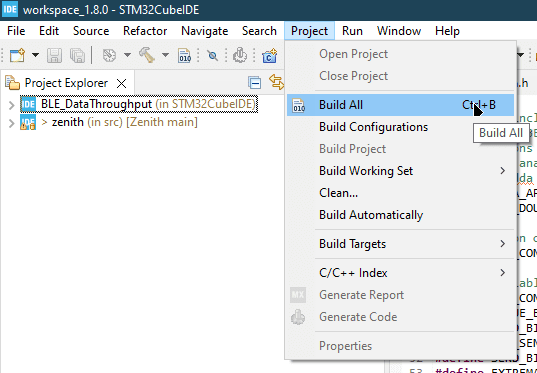
\includegraphics[width=0.6\linewidth]{ide_build.png}
	\caption{STM32CubeIDE building project menu \label{fig:ide_build}}
\end{figure}

\begin{figure}[ht]
	\centering
	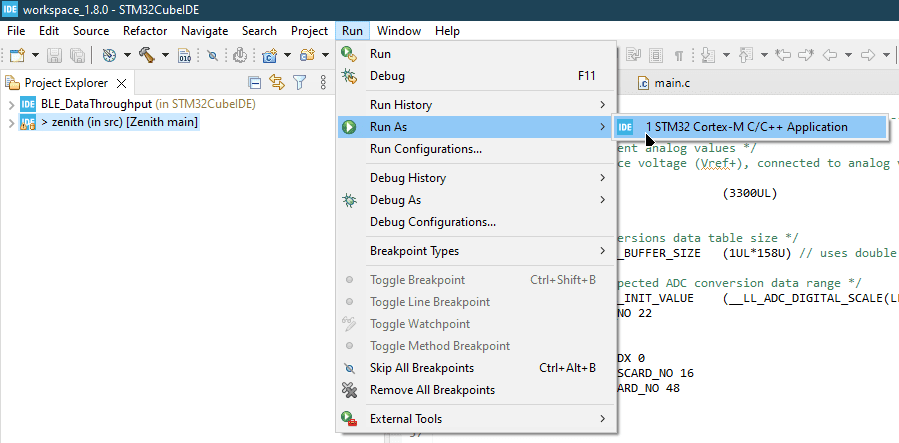
\includegraphics[width=0.8\linewidth]{ide_run.png}
	\caption{STM32CubeIDE running and programming the MCU \label{fig:ide_run}}
\end{figure}

Another way of programming the MCU is with the STM32CubeProgrammer. Connect with the ST-Link connected to the MCU JTAG. On the menu select \textit{Erasing \& Programming} (\cref{fig:prog_program}) and under the \textit{Download} section browse the built binary (this should be located in the project folder under \textit{Release/zenith.elf}). Make sure \textit{Verify before programming} and \textit{Run after programming} are checked. Finally, press \textit{Start Programm...}. If needed, a full MCU program memory erase by clicking on the \textit{Full chip erase} button.

\begin{figure}[ht]
	\centering
	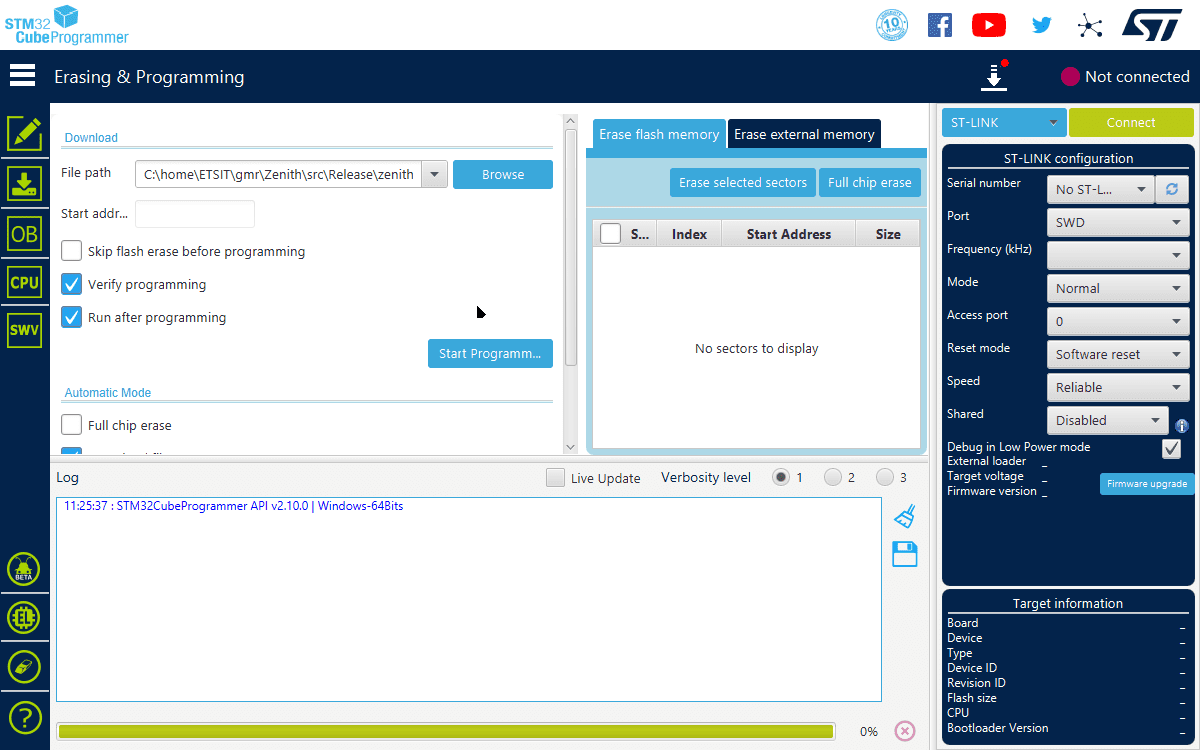
\includegraphics[width=\linewidth]{prog_program.png}
	\caption{STM32CubeProgramming, programming and erasing the MCU \label{fig:prog_program}}
\end{figure}

\section{PC applications preparation}

The PC applications that interface with the node are contained in two Python source files in the PC applications folder. The applications are the following:
\begin{itemize}
	\item \textit{Epsilon Main}: the main application for use in debugging and testing of the ranging characteristic of the radar. It outputs a graph of the bin (distance) to signal strength for every ramp. The source file is \texttt{main.py}.
	\item \textit{Epsilon micro-Doppler}: the application for use in micro-Doppler mode of the radar. It outputs a live STFT graph of the micro-Doppler. The source file is \texttt{main\_md.py}.
\end{itemize}

The Python source files It can be edited with any text based editor, but it is recommended to use \textit{Visual Studio Code}. The installation of \textit{Visual Studio Code} is beyond the scope of this documentation. However, the reader can follow this written tutorial to set up Visual Studio Code for Python development: \url{https://archive.is/tXGq1}.

To execute the PC application when debugging it is also necessary to configure \textit{Visual Studio Code} to select the interpreter that interfaces with \textit{Pipenv}. To do so, open one of the two source code files outlined above and press the key combination \texttt{Ctrl+Shift+P} and type \textit{Select Interpreter} in the command box that pops up. Select the option \textit{Python: Select Interpreter...}; a new box similar to the one shown in \cref{fig:interpreter_select} will show up. Several Python interpreters will show up. Under the interpreters of the \textit{PipEnv} section (look for the \textit{PipEnv} label in the right side), select the one that contains the string \textit{epsilon} in any form. In some instances \textit{Visual Studio Code} will select automatically the correct interpreter when opening up a \textit{pipenv-enabled} project. Nonetheless, it is important to check that the correct interpreter is selected so that the libraries and modules of the PC application load correctly.

A BLE compatible Bluetooth card must be installed and present in the PC before executing any of the available applications. The BLE card during tests and development of the project is a \textit{Qualcomm Atheros QCA61x4 Bluetooth} BLE-enabled card.

\begin{figure}[ht]
	\centering
	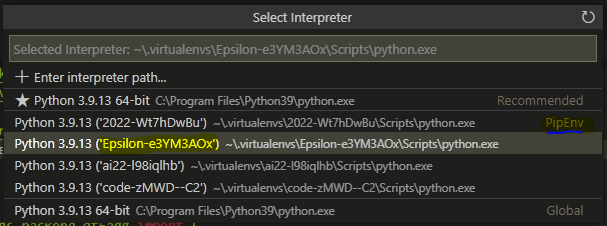
\includegraphics[width=0.9\linewidth]{interpreter_select.png}
	\caption{Python interpreter selection window in \textit{Visual Studio Code} \label{fig:interpreter_select}}
\end{figure}

\section{Main modifications to the PC applications}

As a general rule, the configuration of the PC applications must match that of the firmware.

\subsection{Epsilon Main application configuration}

The configurations available in the main application are as follows:

\begin{minted}{py}
BIN_NO = 20
BIN_START = 90
\end{minted}

These variables must match the following variables configured in the firmware:
\begin{itemize}
	\item $\texttt{BIN\_NO} = \texttt{SEND\_BIN\_NO}$
	\item $\texttt{BIN\_START} = \texttt{SEND\_BIN\_INITIAL\_IDX}$
\end{itemize}

The ramp samples information are stored in a file \texttt{main\_samples.csv} in the same folder of the PC applications.

\subsection{Epsilon micro-Doppler application configuration}

The configurations available in the micro-Doppler application are as follows:

\begin{minted}{py}
SUMS_FFT_SIZE = 20
X_DIM = 200
Y_DIM = SUMS_FFT_SIZE
\end{minted}

Some variables must match the following variables configured in the firmware:
\begin{itemize}
	\item $\texttt{SUMS\_FFT\_SIZE} = \texttt{MD\_BIN\_SUM\_NUMBER}$
\end{itemize}

\texttt{X\_DIM} controls the amount of FFTs of the sums of the ramps that are represented at any given instance, it can be changed to allow the persistence of more STFTs in the screen or shortened to provide a detailed view of a subset of STFTs.

The ramp sums information are stored in a file \texttt{md\_samples.csv} in the same folder of the PC applications.

\section{PC application execution}

After configuring the PC applications, one of the available applications can be executed. Both applications cannot be executed concurrently. To execute any of the applications, in the main folder of the PC applications run:
\begin{minted}{bash}
pipenv run python ***.py
\end{minted}

where \texttt{***.py} is either of \texttt{main.py} or \texttt{main\_md.py}

After executing the applications a window will pop up. The window corresponding to the Main application is shown in \cref{fig:pc_main} and the window corresponding to the microdoppler application is shown in \cref{fig:pc_md}.

\begin{figure}[ht]
	\centering
	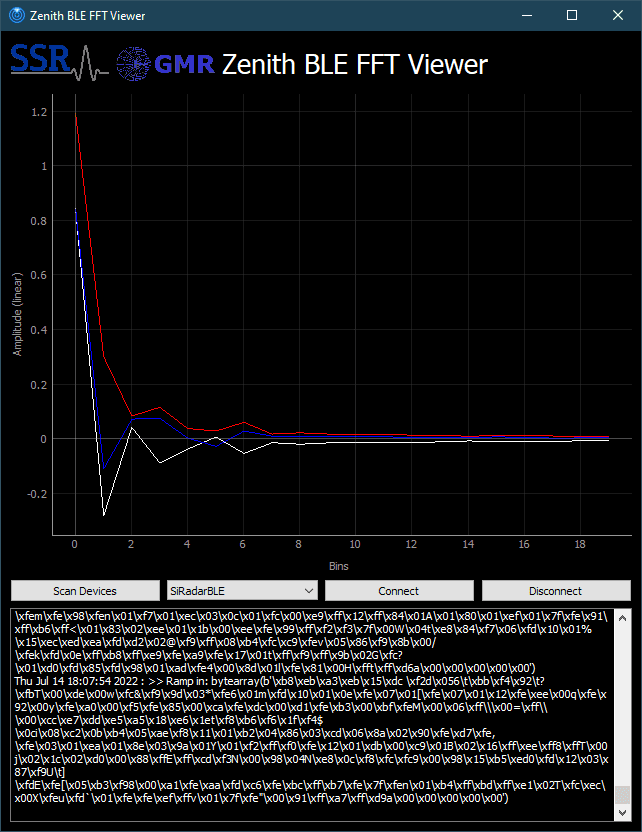
\includegraphics[width=0.8\linewidth]{pc_main.png}
	\caption{Epsilon Main application interface \label{fig:pc_main}}
\end{figure}

\begin{figure}[ht]
	\centering
	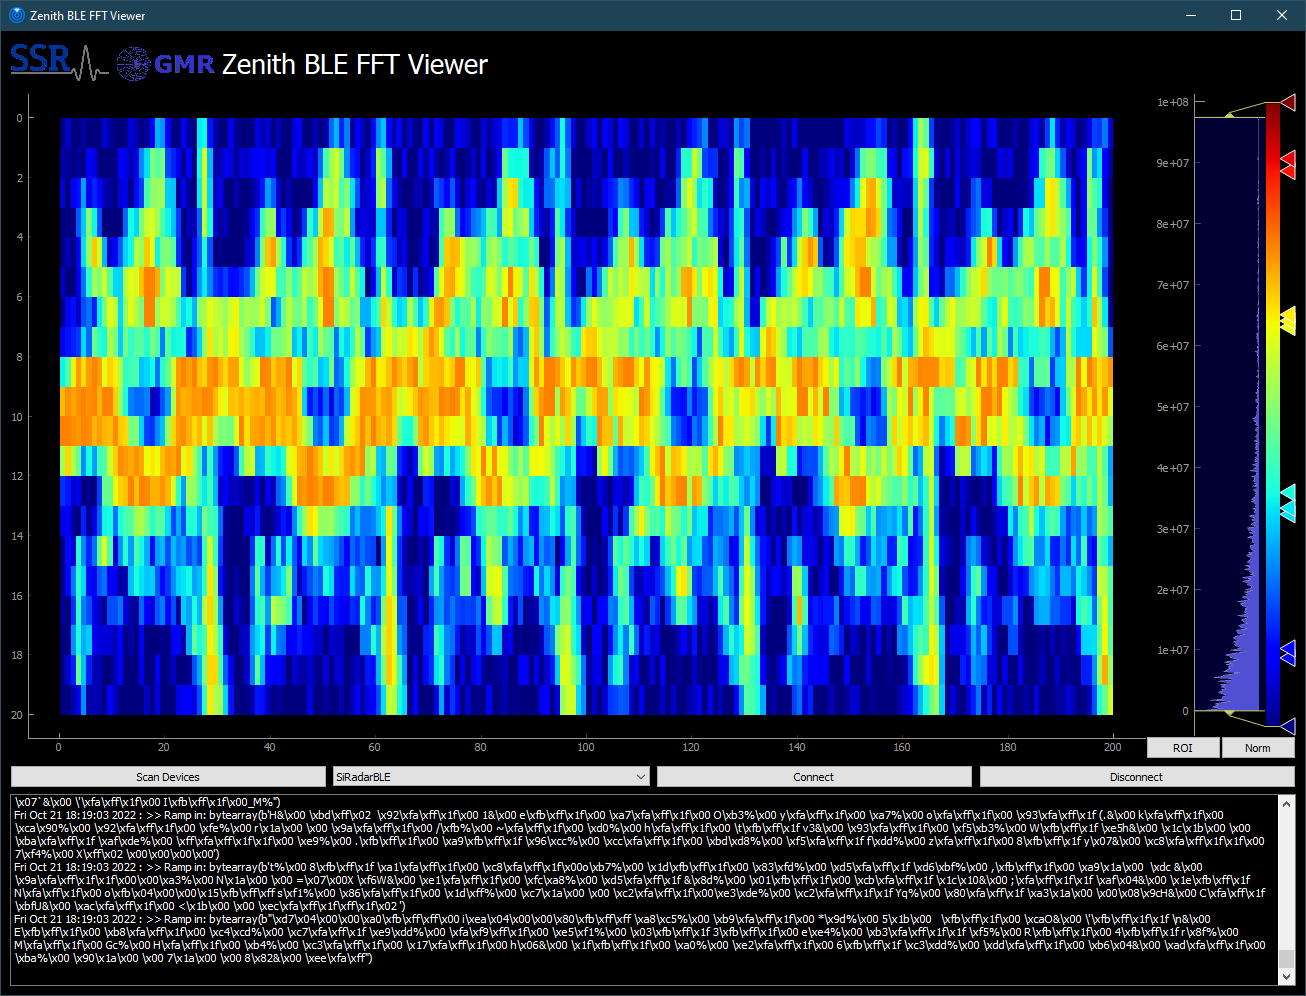
\includegraphics[width=\linewidth]{img/gui_gait.png}
	\caption{Epsilon micro-Doppler application interface \label{fig:pc_md}}
\end{figure}

\section{System execution}

To start the system, first program the MCU with a desired program. Hook up the I and Q signals to their corresponding inputs and connect the trigger. Finally power up the MCU in a stand-alone way.
Then execute any of the PC applications. When the main interface shows up, click the \textit{Scan devices} button. After some seconds some devices will appear in the selectable list next to the button. Select \textit{SiRadarBLE} from that list and click \textit{Connect}.

The system will start receiving and storing samples. To disconnect the system at any time click \textit{Disconnect}. To save an graph image at any time, right click the graph area and select \textit{Export...} a menu will show up where is is possible select the appropriate format and location to store the graph.